\documentclass[a4paper]{article}
\usepackage{cmap}
\usepackage{mathtext}
\usepackage{amssymb}
\usepackage{amsmath}
\usepackage[russian]{babel}
\usepackage{indentfirst}
\usepackage[pdftex]{graphicx}
\usepackage{multirow}
\usepackage{mathrsfs}
\usepackage{biblatex}
\usepackage{siunitx}
\usepackage[left=2cm,right=2cm,top=2cm,bottom=2cm]{geometry}
\usepackage{fancyhdr}
\bibliography{bib}
\pagestyle{fancy}
\newcommand{\rref}[1]{(\ref{#1})}
\newenvironment{comment}{}{}
\newcommand{\picref}[1]{рис. \ref{#1}}
\newcommand{\mbf}{\mathbf}
\newcommand{\Equip}[3]{
	
	{\bf #1:} $\Delta = \pm #2$ \si{#3}}
\newcommand{\equip}[1]{
	
	{\bf #1}}
\newcommand{\labname}{Фазовая дифракционная решётка} 	% название пиши здесь
\newcommand{\labnum}{4.4.2}		% номер вводи здесь
\fancyfoot{}
\fancyhead[RE, RO]{\thepage}
\fancyhead[LE, LO]{Лабораторная работа \labnum \space \labname}
\title{Лабораторная работа \labnum \space \labname} % Название работы здесь
\author{Иван Сладков}
\begin{document}
\maketitle
\thispagestyle{empty}
\section{Аннотация}
В данной работе проводится  знакомство с работой и настройкой гониометра Г5, определение спектральных характеристик фазовой решётки (эшелетта) и исследование спектра ртутной лампы.

\section{Теоретические сведения}

\begin{figure}[tbp]
	\centering
	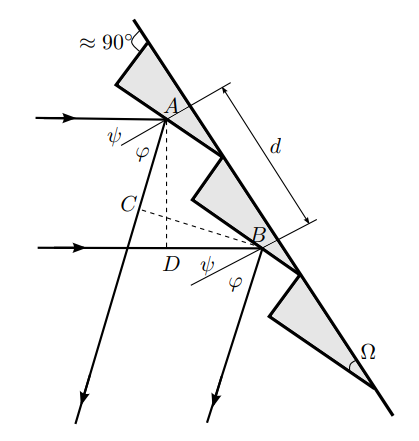
\includegraphics[width=0.8\linewidth]{Screenshot_2}
	\caption{Профиль фазовой дифракционной решётки; дифракция световой волны}
	\label{fig:решёткаВпрофиль}
\end{figure}

В современных спектральных приборах широко используются отражательные решётки с треугольным профилем штриха (рис. \ref{fig:решёткаВпрофиль}), они способны концентрировать до $ 70–80\% $ падающего излучения в рабочий порядок спектра. Отражательная решётка, в которой угол $ \Omega $ между рабочей гранью и плоскостью решётки не превышает $ 20^\circ $, называется эшелеттом. Для эшелетта, варьируя угол скоса и шаг решётки, получают рабочий порядок $ m_р \le 10 $.

Найдём разность хода между лучами на рис. \ref{fig:решёткаВпрофиль}. Условие возникновения спектра порядка $ m $:
\begin{equation}\label{eq:spectreM}
	A C - B D = d (\sin \varphi m- \sin \psi) = m \lambda,
\end{equation}
где $ \psi $ -- угол падения от нормали к решётке, $ \varphi $ -- угол дифракции.
Для нулевого порядка $ \varphi_0 = \psi $. В отличие от амплитудной решётки, нулевой порядок не будет самым ярким. Угол $ \varphi_б $ -- угол блеска, соответствующий максимуму интенсивности света, равен углу зеркального отражения падающей волны от одной ступеньки:
\begin{equation*}\label{key}
	\varphi_б = \psi+ 2 \Omega.
\end{equation*}
Для эшелетта рабочим порядком спектра $  m_р$ будет то целое число, которое соответствует минимальной ошибке решения уравнения $d \sin \varphi_m - \sin \psi = 0 $.

Cчитая, что эшелетт работает в автоколлимационном режиме, то есть свет падает перпендикулярно рабочей грани решётки ($ \psi = -\Omega $) и отражается в обратном направлении ($ \varphi = \Omega $), тогда
\begin{equation}\label{om}
	2 d \sin \Omega = m_р \lambda_р.
\end{equation}
В автоколлимационном режиме дифракция на одной ступеньке-зеркальце описывается так же, как и дифракция на отдельной щели амплитудной решётки с максимумом вблизи $ \varphi \approx 0 $. В отличие от амплитудной решётки, нумерацию порядков для амплитудной решётки, следует сместить на величину $ m_р $.

\subsection{Расчётные формулы}

Основные формулы, используемые в работе: \eqref{eq:spectreM}, \eqref{om}. Вторая часть формулы (1) используется для определния периода $ d $ в МНК на графике рис. 2.

\section{Оборудование и инструментальные погрешности}

\Equip{Гониометр}{1}{''}
\equip{Эшелетт}: $ \lambda_р = \SI{500}{\nano \metre} $ в 1-м порядке.
\equip{Ртутная лампа}

\section{Результаты измерений и обработка данных}
\emph{Все измерения и расчёты в СИ.}

Линии спектра лампы были исследованы для угла $ \phi = 45^\circ $. Результаты отображены в табл. \ref{tab:allspectre}.
\begin{table}[htb]
	\centering
\begin{tabular}{|c|c|c|}
	\hline
	Цвет       & $ \sin\varphi -\sin\psi $ & $ \lambda$ \\ \hline
	Фиолетовый & -0.249                  & 4047       \\ \hline
	Синий      & -0.267                   & 4358       \\ \hline
	Голубой    & -0.301                  & 4916       \\ \hline
	Зелёный    & -0.331                  & 5461       \\ \hline
	Жёлтый     & -0.353                  & 5770       \\ \hline
	Жёлтый     & -0.354                  & 5791       \\ \hline
\end{tabular}
\caption{Спектр ртути}
\label{tab:allspectre}
\end{table}

По этим данным построим график на рис. \ref{fig:screenshot1}.
\begin{figure}[tbp]
	\centering
	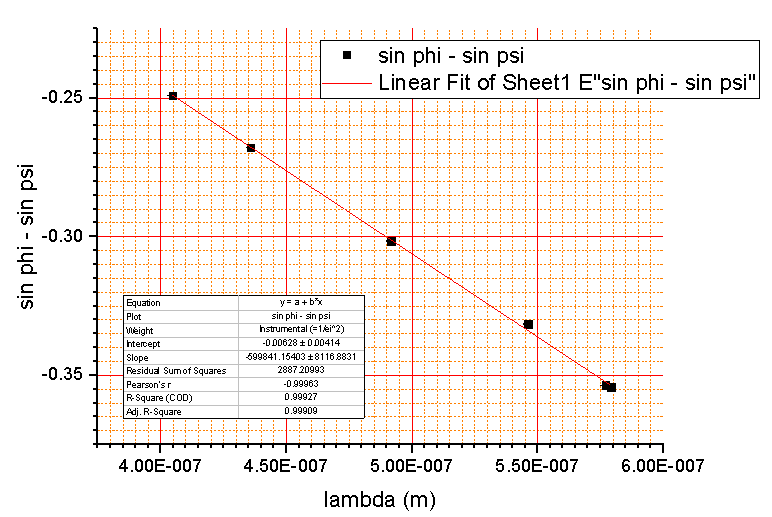
\includegraphics[width=0.8\linewidth]{Screenshot_1}
	\caption{График $\sin \varphi - \sin \psi$ от $\lambda$}
	\label{fig:screenshot1}
\end{figure}
Отсюда 
\begin{equation*}\label{key}
	\frac{1}{d} = 599 \pm 8\; штр/мм.
\end{equation*}
\begin{equation*}\label{key}
	d = 1.67 \pm 0.08 \; мкм/штр.
\end{equation*}

Найдём угол скоса рабочей поверхности: $ m_р = 1 $, $ \lambda_р = 500 \; нм $, тогда
\begin{equation*}\label{key}
	\sin \Omega = \frac{m_р \lambda_р}{2 d} = 0.150\pm 0.005
\end{equation*}
\begin{equation*}\label{key}
	\Omega = 8.61^\circ \pm 0.02^\circ.
\end{equation*}

Найдём угловую дисперсию при различных $ \psi $. Результат в табл. \ref{tab:dispersion}. Удалось снять только по 1 порядку для $\varphi = 45^\circ$ и $ \varphi = 60^\circ $, и 2 порядка для $ \varphi = 30^\circ $, так как для остальных $ m $, характерные углы превышают максимально измеримые.



\begin{table}[]
	\centering
	\begin{tabular}{|l|l|l|l|l|}
		\hline
		$\varphi$ &
		$\left|\Delta \varphi\right|$ &
		$\Delta \lambda$, \AA{} &
		$\left|\frac{d \varphi}{d \lambda}\right|_{эксп}$, (угл. с./\AA{}) &
		$\left|\frac{d \varphi}{d \lambda}\right|_{теор}$, (угл. с./\AA{}) \\ \hline
		$30^\circ$ & $650\pm 10$  & $21$ & $31\pm 1$ & $1.5\pm 0.05$ \\ \hline
		$30^\circ$ & $798\pm 10$  & $21$ & $38\pm 1$ & $1.55\pm 0.05$ \\ \hline
		$45^\circ$ & $1286\pm 10$ & $21$ & $61\pm 1$ & $2.5\pm 0.1$     \\ \hline
		$60^\circ$ & $1441\pm 10$ & $21$ & $68\pm 1$ & $4.4\pm 0.2$     \\ \hline
	\end{tabular}
	\caption{Угловая дисперсия при различных $ \varphi $}
	\label{tab:dispersion}
\end{table}

Построим график для угловой дисперсии при $ \varphi = 30^\circ $.

\begin{figure}[tbp]
	\centering
	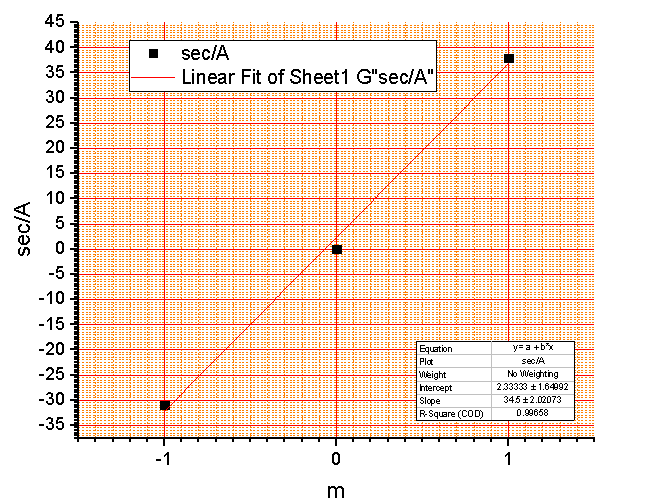
\includegraphics[width=0.8\linewidth]{Screenshot_3}
	\caption{Угловая дисперсия для $30^\circ$}
	\label{fig:screenshot3}
\end{figure}

\subsection{Оценка разрешающей способности}

Найдём экспериментальную разрешающую способность системы при ширине щели 1.14 мм:
\begin{equation*}\label{key}
	R = \frac{\lambda}{\delta \lambda} = 274.7.
\end{equation*}
Тогда $ N =275 $ штрихов освещены. Так как коллиматор даёт параллельный пучок, то на 1 мм приходится $ n\approx 250 $ штрихов. Оценка погрешности не имеет смысла, так как такой метод в принципе неточен и опирается на субъективную оценку.

\subsection{Оценка погрешностей}

Как и обычно, оценка инструментальных погрешностей проводится по общей формуле (с частными производными); в экспериментах с несколькими измерениями случайные погрешности существенно превалируют над инструментальными. 

\section{Вывод}

Судя по расхождению экспериментальных данных с теоретическими, при снятии показаний гониометра, несмотря на его точность, были допущены ошибки, в частности, при измерении расстояния между жёлтыми спектральными линиями. Отчасти это связано с неудобством снятия показаний.

Тем не менее, удалось с неплохой точностью найти характеристики дифракционной решётки и исследовать спектр ртутной лампы.

\newpage
\begin{thebibliography}{9}
	\bibitem{Siv} Сивухин Д. В. \emph{Общий курс физики. Том 4 Оптика}, 2004
	\bibitem{kir} Кириченко Н. А. \emph{Принципы оптики}, 2014
	\bibitem{max} \emph{Лабораторный практикум по общей физике. В 3 томах. Том 2. Оптика: учебное пособие} под ред. А. В. Максимычева
\end{thebibliography}
\end{document}